\documentclass{article}
\usepackage[french]{babel}
\usepackage[a4paper,top=2cm,bottom=2cm,left=3cm,right=3cm,marginparwidth=1.75cm]{geometry}

\usepackage{amsmath}
\usepackage{float}
\usepackage{graphicx}
\usepackage[colorlinks=true, allcolors=blue]{hyperref}
\usepackage{listings}

\begin{document}
\begin{titlepage}
\begin{center}

\vspace*{2cm}

\Huge \textbf{Rapport de projet}\\
\vspace{0.5cm}
\Large \textbf{UE Projet MIDL 2}\\

\vspace{1cm}

\large Auteurs \\ \textbf{Chloé Godart -- Noé Mastrorillo -- Théophile Sochard}\\
\vspace{0.5cm}
Formation \\ \textbf{L3 MIDL}


\vspace{1cm}


\large Professeurs \\ \textbf{Emmanuelle Claeys -- Mathieu Sablik}

\vspace{1cm}


\includegraphics[width=0.5\linewidth]{assets/Logo_UT3.jpg}


\vspace{1cm}

Lundi 13 Janvier 2025

\vspace{1cm}

\href{https://github.com/theosoch/projet-midl-2.git}{Lien GitHub}
 \\
\href{https://colab.research.google.com/drive/1JksiwP0xOu8adagP3vgTN8qdQLHjGTxZ?usp=drive_link}{Lien Google Colab}


\end{center}
\end{titlepage}

\newpage
\tableofcontents
\newpage
\section{Introduction}
Ce rapport présente notre travail pour le projet MIDL 2, ayant pour but l'analyse des données recueillies lors des JO Tokyo 2020 et Paris 2024. 
\\

Nous explorerons d'abord les données à l'aide de méthodes statistiques, ce qui nous permettra par exemple de comparer les tendances anticipées grâce à cette analyse, aux résultats obtenus grâce au modèle. Ensuite, nous tenterons donc de mettre en place un modèle prévoyant le nombre de médailles par pays pour les JO 2024. A partir de ce modèle, et en utilisant des données légèrement différentes, nous essaierons également de mesurer l'impact de la non-participation de la Russie lors des JO Paris 2024. 
\\

Enfin nous nous intéresserons aux variables socio-économiques expliquant le succès d'un pays aux JO, que nous pouvons mesurer grâce au nombre de médailles et au classement global.
\\

Plutôt que de séparer ce rapport en 2 parties : analyse exploratoire et modélisation, il s'organisera autour de problématiques auxquelles nous essaierons de répondre, puisque ces 2 étapes se complètent en pratique.
\\

\section{Analyse exploratoire}

Cette  partie concerne seulement quelques premières observations que nous pouvons faire à partir des données. Elles n'ont pas pour but de répondre à une problématique. 

\subsection{Parité, nombre de participants par pays}

Intéressons-nous à l'évolution de la répartition de certains critères, tels que la parité ainsi qu'au nombre de participants par pays.
\\

Les informations nécessaires sont présentes dans le fichier \verb|athletes.csv|. Pour le nombre de participants par pays, nous pouvons anticiper une évolution notable pour les pays hôtes, ce qui est confirmé dans la figure 1.

\begin{figure}[H]
    \centering
    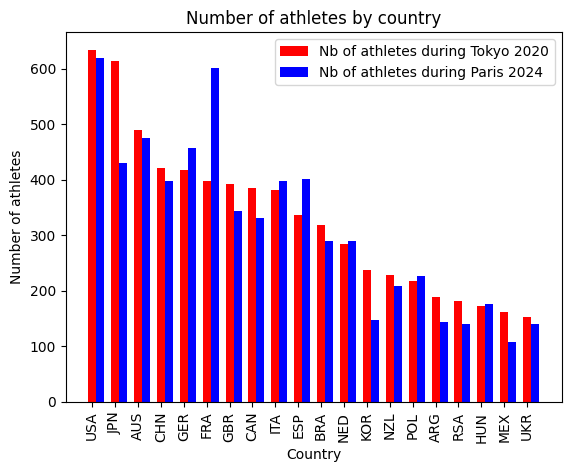
\includegraphics[width=0.75\linewidth]{assets/nb_participants_by_country.png}
    \caption{Evolution du nombre de participants par pays entre 2020 et 2024}
    \label{fig:enter-label}
\end{figure}

Nous remarquons bien des valeurs très différentes pour la France et le Japon. Cela est en particulier dû au fonctionnement des qualifications pour le pays hôte : en effet, il bénéficie de certains quotas (qualifications d'office) maximums par discipline, facilitant la participation d'un plus grand nombre d'athlètes. De plus, nous observons un écart marqué par exemple pour la Corée du Sud (KOR) qui a plus participé aux JO de Tokyo ou l'Espagne (ESP) qui a plus participé à ceux de Paris. Nous pourrions donc supposer qu'il y a un facteur de proximité au pays hôte qui influence le nombre de participants par pays.
\\

Les pays ne participant pas aux deux éditions des JO sont bien sûr exclus puisque nous ne pouvons pas comparer les données. Nous utilisons pour ce graphique une jointure de deux dataframes contenant les nombres d'athlètes par pays de 2020 et 2024, la fonction merge n'inclut donc pas les pays qui n'apparaissent pas dans les deux dataframes.
\\

Pour la proportion hommes/femmes au sein des athlètes, nous avons pratiquement la parité aux deux éditions des JO (Tokyo 52.2 47.8, Paris 50.9 49.1), nous remarquons une légère amélioration. Les fonctions utilisées pour compter le nombre d'athlètes ignorent les valeurs manquantes, les athlètes dont nous ne connaissons pas le genre sont donc exclus de ces statistiques.
\\

Nous pouvons également nous intéresser à cette proportion par pays.

\begin{figure}[H]
    \centering
    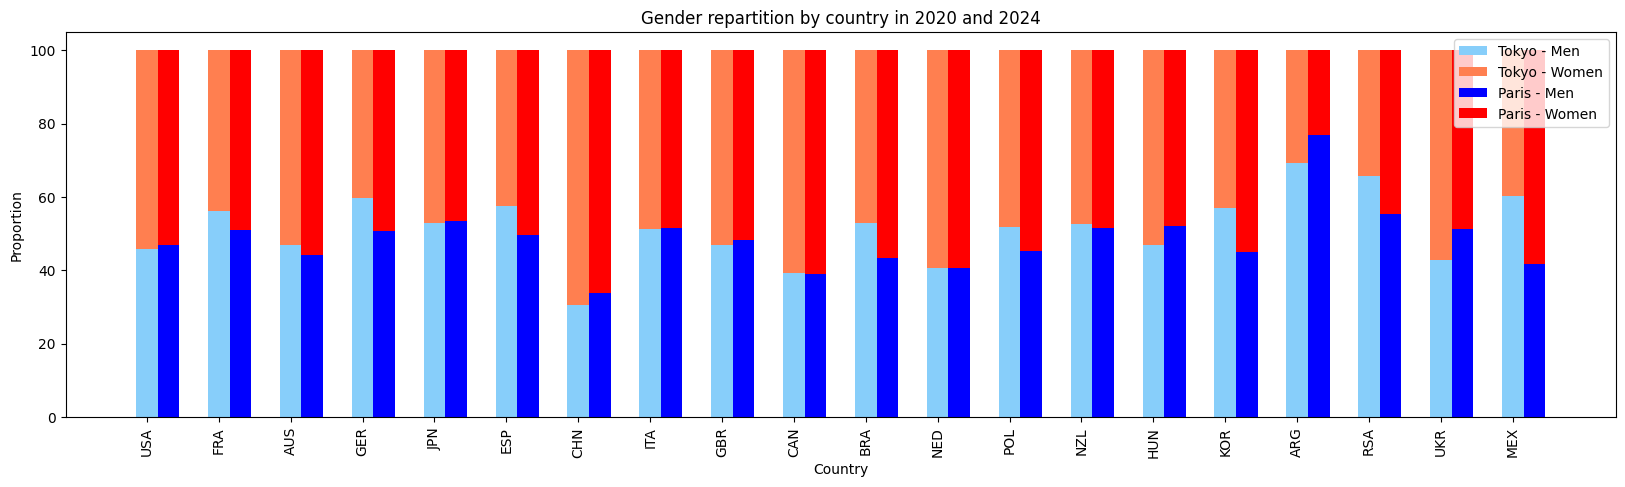
\includegraphics[width=1\linewidth]{assets/parite_pays.png}
    \caption{Evolution de la proportion hommes/femmes par pays entre 2020 et 2024}
    \label{fig:enter-label}
\end{figure}

Ici, seulement les 20 pays ayant le plus de participants sont affichés. Les proportions variables s'expliquent par les disciplines pour lesquelles se sont qualifiés les athlètes. Par exemple, l'Argentine (ARG) présente une grande proportion d'athlètes masculins car l'équipe masculine de football s'est qualifiée, contrairement à l'équipe féminine. Idem pour la Chine (CHN) où, en revanche, les athlètes féminines sont plus qualifiées de manière globale et pas dans un sport spécifique.

\subsection{Pourcentage d'athlètes médaillés en fonction du nombre de disciplines médaillées}

Enfin, nous avons trouvé intéressant d'étudier la relation entre le pourcentage d'athlètes médaillés et le nombre de disciplines médaillées par pays. Vous pouvez retrouver les graphiques en annexe \ref{annexe_athletes_disciplines}. Nous noterons ici que nous avons exclu les pays qui n'ont pas récolté de médailles.
\\

Dans ces deux graphiques, nous pouvons identifier plusieurs groupes. Dans la partie droite se trouvent les pays qui ont été très performants aux Jeux Olympiques, avec beaucoup de disciplines médaillées. Nous y retrouvons notamment les Etats-Unis d'Amérique qui ont brillé aux deux JO, la Grande-Bretagne, la Chine, la France ou encore la Russie pour 2020.
\\

Dans la partie supérieure gauche, ce sont les pays qui sont très spécialisés, avec très peu de disciplines médaillées mais un grand effectif de leurs athlètes médaillés. Nous y retrouvons par exemple les Fidji en 2020 avec une seule discipline médaillée (le rugby à sept) et près de 80\% de leurs athlètes médaillés.
\\

Enfin, nous retrouvons un groupe homogène dans la partie inférieure gauche qui représente les pays qui n'ont pas vraiment brillé aux Jeux Olympiques, avec peu de disciplines médaillées et une petite proportion d'athlètes médaillés.
\\

Pour confirmer cette analyse, nous avons décidé d'utiliser un modèle de clustering KMeans qui va identifier les trois groupes précédents. Ce modèle nous permettra de mieux voir les mouvements entre les groupes aux JO 2024 par rapport aux groupes des JO 2020. Nous avons tout d'abord standardisé nos données pour qu'elles suivent une distribution normale centrée réduite afin d'avoir la même échelle sur les deux axes, puis nous avons pu entraîner le modèle qui nous a donné les clusters que vous pouvez retrouver dans le graphique en annexe \ref{annexe_athletes_disciplines_clusters}.
\\

Dans ce graphique, le cluster rouge représente le groupe des pays très spécialisés dans quelques disciplines (que nous numéroterons 0), le cluster vert représente le groupe des pays très performants (numéroté 1), et le cluster bleu représente le groupe général des pays qui n'ont pas été très performants (numéroté 2).
\\

Nous avons également utilisé une matrice de confusion entre les clusters de 2020 et de 2024 pour identifier les mouvements de groupes entre les deux Jeux Olympiques, comme le montre la figure suivante.

\begin{figure}[H]
\begin{center}
    \begin{tabular}{|c|c|c|c|c}
    \hline
        Paris & 0 & 1 & 2  \\
        Tokyo &   &   &    \\
        \hline
        0     & 2 & 0 & 12 \\
        \hline
        1     & 0 & 9 & 5  \\
        \hline
        2     & 4 & 0 & 37 \\
        \hline
    \end{tabular}
\end{center}
\caption{Matrice de confusion entre les clusters de Tokyo 2020 et Paris 2024}
\label{fig:enter-label}
\end{figure}

Plusieurs choses intéressantes sont à observer ici. Tout d'abord, seulement 2 pays qui étaient dans le groupe des pays spécialisés en 2020 y sont restés en 2024, là où les 12 autres sont passés dans le groupe général. Pour les pays qui étaient dans le groupe des pays très performants en 2020, 9 sont restés et les 5 autres sont également passés dans le groupe général. Enfin, 4 pays qui étaient dans le groupe général en 2020 sont passés dans le groupe spécialisé en 2024.

\section{Prediction du nombre de médailles par pays}
Dans cette section, l'objectif est d'essayer de trouver des facteurs pouvant expliquer l'évolution du classement des médailles aux JO de Paris par rapport à ceux de Tokyo.

\subsection{Evolution du classement des médailles par pays}
Pour étudier le classement de manière globale, nous pouvons nous restreindre au nombre total de médailles de tout type (bronze, argent, or) par pays. Les données relatives au nombre total de médailles par pays se trouvent dans le fichier \verb|medals_total.csv|. Ainsi, nous pouvons visualiser l'évolution de ce nombre de médailles par pays lors des deux jeux (cf. annexe \ref{annexe_comp_nb_total_medailles_par_pays}).
\\

A partir de ces informations, nous pouvons nous intéresser à deux principaux facteurs possibles, l'influence du pays hôte et l'impact de la non-participation d'un des pays les plus importants des JO de Tokyo par sa place de 3ème dans le classement de ces jeux, la Russie.

\subsubsection{Impact du pays hôte}

Les pays hôtes des jeux de Tokyo et de Paris sont respectivement le Japon et la France. Nous pouvons nous attendre à ce que ces pays aient un avantage/désavantage à accueillir les compétitions. Pour mesurer cet effet, nous pouvons simplement comparer leur nombre de médailles entre les deux jeux. Pour le Japon, nous pouvons alors nous attendre à une diminution de son nombre de médailles lors des jeux de Paris et, au contraire, à une augmentation du nombre de médailles pour la France.

\begin{figure}[H]
    \centering
    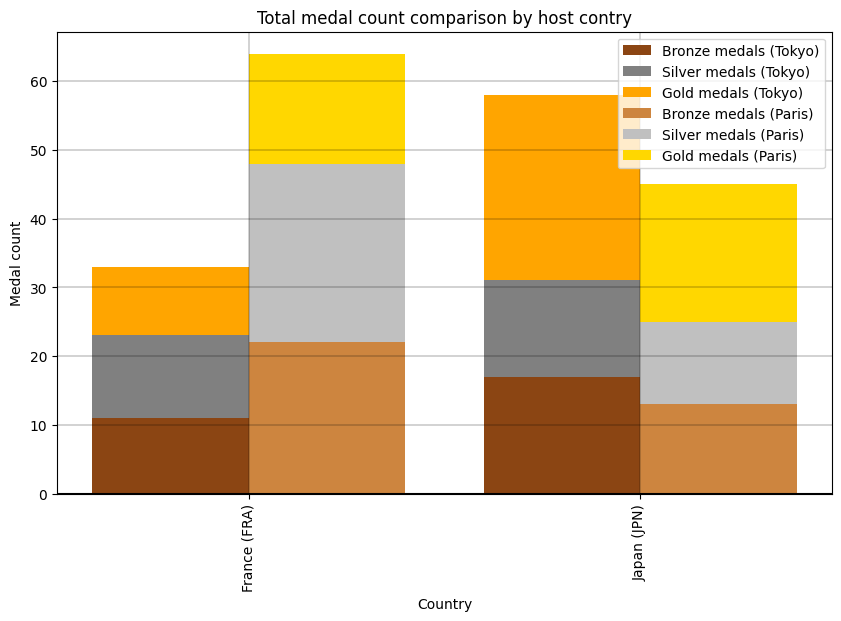
\includegraphics[width=0.6\linewidth]{assets/comp_nb_total_medailles_pays_hotes.png}
    \caption{Comparaison du nombre total des médailles des pays hôtes}
    \label{fig:enter-label}
\end{figure}

Nous constatons bien les différences de nombre de médailles attendues, avec une diminution légère pour le Japon (JPN) qui s'explique sûrement par sa performance lui permettant de surpasser le désavantage de ne pas être le pays hôte. La raison de cet avantage/désavantage est celle expliquée plus haut.

\subsection{Evolution de la répartition des médailles par continent}

Après avoir étudié les variations par pays, on peut se demander si ces variation ont impacté le classement des continents. Le graphique suivant montre le nombre de médailles de bronze, d'argent et d'or ainsi que le total pour chaque continent aux JO 2020 (barres de gauche) et 2024 (barres de droite)

\begin{figure}[H]
    \centering
    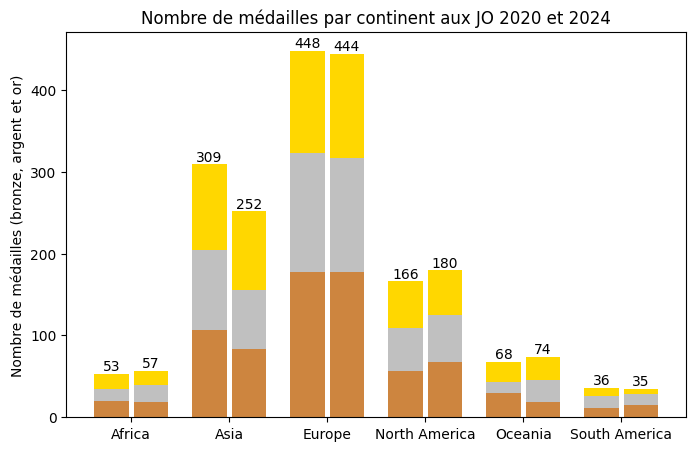
\includegraphics[width=0.6\linewidth]{assets/medals_continents.png}
    \caption{Nombre de médailles par continent aux JO 2020 et 2024}
    \label{fig:enter-label}
\end{figure}

Nous avions le choix de placer la Russie en Europe ou en Asie et nous avons choisi l'Asie car c'est le continent dans lequel elle a le plus de superficie. Cela explique donc la grosse chute du nombre de médailles de l'Asie entre les JO 2020 et 2024, puisqu'en 2024 la Russie n'a pas eu le droit de participer aux Jeux Olympiques de Paris. Nous pourrions également justifier cette chute par la diminution du nombre de médailles du Japon.
\\

En ce qui concerne les autres continents, il n'y a pas de différence très notable. L'Afrique, l'Amérique du Nord et l'Océanie ont augmenté leur score de quelques médailles aux JO 2024, l'Europe et l'Amérique du Sud ont quant à eux perdu quelques médailles entre les deux Jeux Olympiques. Bien que ces différences ne soient pas très importantes, il est surprenant que l'augmentation du nombre de médailles de la France n'ait pas fait augmenter celui de l'Europe, qui a même légèrement diminué. Le type des médailles est aussi assez similaire en 2020 et 2024, sauf pour l'Océanie qui a récolté d'avantage de médailles d'argent et d'or à Paris, là où elle avait beaucoup de bronze à Tokyo.

\subsection{Modèle prédictif}

Il nous a paru intéressant d'essayer de créer un modèle prédictif nous permettant de prédire le classement des pays aux jeux de Paris à partir des données des jeux de Tokyo. Pour ce faire, nous avons dû tester plusieurs types de modèles différents afin d'établir lequel serait le plus intéressant/performant.
\\

L'objectif est de créer un modèle de prédiction de la médaille qu'un athlète, étant donné ses caractéristiques, obtiendrait lors d'une épreuve pour une discipline donnée.
\\

Ainsi, en sachant a quel pays appartient chaque athlète, nous pourrons sommer les résultats des athlètes par pays et obtenir un classement que nous pourrions comparer au classement réel.

\subsubsection{Traitement des données}

La première difficulté rencontrée a été les données. En effet, les données des jeux de Tokyo fournies étaient lacunaires ou inexploitables en l'état. Il nous a donc paru plus simple de récupérer d'autres données, plus complètes depuis internet. Pour ce faire, nous nous sommes servis du site \href{https://www.olympedia.org/}{Olympedia} et avons créé un script Python afin de récupérer les résultats des athlètes et leurs caractéristiques par pays, dans chaque épreuve (événement), dans chaque discipline.
\\

Les données des jeux de Paris étaient plus complètes mais devaient tout de même être fortement transformées pour être exploitées.
\\

Au final, parmi les données récoltées et après mise en commun entre les données de Paris et de Tokyo, nous avons établi la liste de features suivantes pour entraîner notre modèle: la discipline, l'âge de l'athlète, le sexe de l'athlète, la taille de l'athlète et le poids de l'athlète. Une autre feature aurait pu être utilisée, à savoir le code du pays de l'athlète, mais après réflexion et avoir testé, il se trouve que cela incite le modèle à renforcer les performances passées des pays, ce que nous aimerions éviter pour prédire le plus impartialement possible les résultats de Paris.
\\

Nous avons aussi dû exclure les pays n'ayant pas participé aux deux éditions des JO pour que le modèle soit capable d'estimer des résultats non influencés par les résultats de ces pays lors des jeux de Tokyo. En effet, ces pays ne participant pas lors des jeux de Paris, ils ne devraient pas avoir d'incidence sur les résultats des pays participants. Les pays ayant participé aux jeux de Paris mais pas à ceux de Tokyo ne peuvent pas être prédits non plus, nous les avons donc aussi exclus.

\subsubsection{Modélisation}

Avant de pouvoir utiliser nos données pour créer nos modèles, il nous a fallu transformer certaines données qualitatives: la discipline, le sexe et la médaille obtenue par l'athlète.
\\

Comme dit précédemment, nous avons testé plusieurs types de modèles prédictifs: des modèles qualitatifs et quantitatifs d'arbres décisionnels et de régressions.

\subparagraph{Arbres décisionnels}
\ \\

Pour les arbres décisionnels, nous avons décidé de tester les arbres décisionnels régressifs et les arbres décisionnels de classification jusqu'à une profondeur de \verb|25|. Voici les scores (par cross-validation) obtenus:

\begin{figure}[H]
    \centering
    
    \caption{Scores des arbres décisionnels régressifs}
    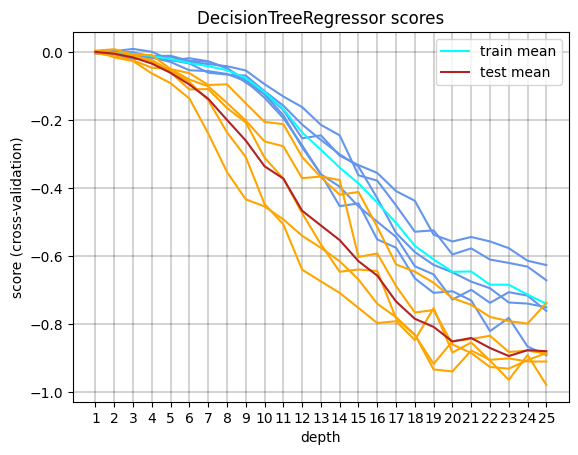
\includegraphics[width=0.6\linewidth]{assets/regressor.decision_tree.scores.png}
\end{figure}
\begin{figure}[H]
    \centering
    
    \caption{Scores des arbres décisionnels de classification}
    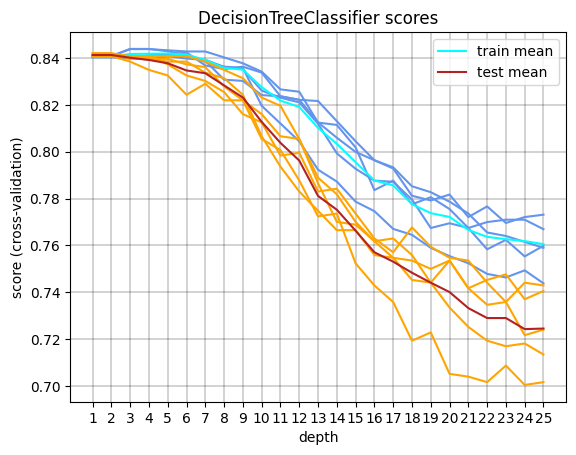
\includegraphics[width=0.6\linewidth]{assets/classifier.decision_tree.scores.png}
\end{figure}

Nous en déduisons rapidement que le meilleur modèle d'arbre est un modèle de classification.
D'après les résultats obtenus, le modèle d'arbre décisionnel de classification le plus en good-fit est celui de profondeur \verb|6|.

\subparagraph{Régressions}
\ \\

Pour les régressions, nous avons décidé te tester une régressions linéaire et une régression logistique. Voici les scores moyens (par cross-validation) obtenus:

\begin{figure}[H]

\caption{Scores de précision moyens des modèles de régression}
\begin{center}
\begin{tabular}{|c|c|c|}
     \hline
     Model               & Train score mean & Test mean score \\
     \hline
     Linear Regression   & $\approx$\verb|0.002| & $\approx$\verb|0.004| \\
     Logistic Regression & $\approx$\verb|0.841| & $\approx$\verb|0.843| \\
     \hline
\end{tabular}
\end{center}

\end{figure}

De même que pour les arbres, nous constatons immédiatement que la régression linéaire n'est pas du tout adaptée.

\subparagraph{Choix du modèle}
\ \\

Le meilleur modèle d'arbre et la régression logistique sont à peu près équivalents. Cependant, en définitive, l'arbre décisionnel de classification de profondeur 6 nous semblait plus adapté à notre problème, nous avons donc arbitrairement choisi d'utiliser ce modèle.

\subparagraph{Prédictions des résultats de Paris}
\ \\

Dans un premier temps nous pouvons noter que le modèle prédit les résultats des athlètes avec \verb|84%| de précision. Lorsque nous en déduisons un classement, voici le top 10 que nous obtenons comparé au top 10 réel:
\begin{figure}[H]

\caption{Tableau de comparaison top 10 prédit vs. réel du classment par médailles des pays}
\begin{center}
\begin{tabular}{|c|c|c|}
     \hline
     Rank & Predicted     & Real \\
     \hline
     1    & Japan         & United States \\
     2    & France        & China \\
     3    & United States & Netherlands \\
     4    & Germany       & France \\
     5    & Australia     & Great Britain \\
     6    & Spain         & Spain \\
     7    & Puerto Rico   & Australia \\
     8    & South Sudan   &	Italy \\
     9    & Brazil        & Japan \\
     10   & Serbia        & New Zealand \\
     \hline
\end{tabular}
\end{center}

\end{figure}

Nous constatons que le classement prédit n'est pas très ressemblant à la réalité. Cependant, nous retrouvons une grande partie des pays présents dans le top 10 réel (Japon, France, Etats-Unis, Australie, Espagne).
\\

Pour essayer de comprendre pourquoi notre modèle manque de précision, nous pouvons nous intéresser à la répartition des types de médailles prédit. En effet, nous constatons alors que la répartition réelle est d'environ \verb|1/3| pour chaque type de médaille (bronze, argent, or) contre une répartition de \verb|0%| de médailles d'or,  $\approx$\verb|72%| d'argent et $\approx$\verb|28%| de bronze. De plus, le nombre total de médailles prédit, tout types et pays confondus (soit sur l'ensemble des jeux) est de \verb|138| contre \verb|2301| en réalité. Notre modèle semble donc ne pas arriver à respecter les règles de répartition des médailles en n'hésitant pas à attribuer peu de médailles et en concentrant leur répartition sur les médailles d'argent quitte à faire des ex-aequo.
\\

Deux hypothèses pourrait expliquer ces problèmes:
\\

\indent\indent 1. Notre jeu de données est trop petit et manque de précision, notamment sur les épreuves, les équipes, l'adversaire lors de l'épreuve, etc. Notre modèle pourrait donc certainement être amélioré en utilisant un plus grand nombre de données et d'indicateurs, notamment historiques, soit des jeux précédents (jusqu'à 3 ou 4 jeux en arrière par exemple).
\\

\indent\indent 2. Lorsque nous regardons les proportions d'athlètes n'ayant pas reçu de médailles dans les données réelles aussi bien de Tokyo que de Paris, cela représente une très large majorité des athlètes. Ceci explique en partie la précision du modèle qui n'a que peu de chance de se tromper en prédisant qu'un athlète n'ait pas reçu de médaille. Il serait alors intéressant d'entrainer le modèle en attribuant une importance, sous forme de poids par exemple, aux valeurs les moins représentatives, bien que nécessaires. Toujours est-il qu'il faudrait alors trouver les bons poids.

\section{Mesure de l'impact de la non-participation de la Russie en 2024}
La Russie a participé aux JO de Tokyo 2020 sous le nom de "Russian Olympic Committee" (ROC) mais pas à ceux de 2024 suite à la guerre en Ukraine. La Russie a remporté 71 médailles en 2020, dont 20 en or, nous pouvons donc nous demander si son absence a impacté notablement le classement global en 2024.

\subsection{Evolution du classement général en étudiant la non-participation de la Russie}

L'impact de la non-participation de la Russie au JO de Paris peut se mesurer en partie à travers l'évolution global du nombre de médailles par pays.
\\

Pour cela, nous avons regardé la somme des différences de médailles par pays entre les jeux de Paris et ceux de Tokyo en excluant la Russie. Ainsi, si le résultat est positif, cela signifie que les pays ont globalement gagné des médailles par rapport aux jeux de Tokyo et au contraire, si le résultat est négatif, ils ont alors globalement perdu des médailles.
\\

Après calcul, nous constatons une augmentation globale du nombre de médailles de `34` médailles. La non-participation de la Russie a bel et bien eu un impact: l'effet de sa non-participation est que ses médailles on été réparties (d'une manière ou d'une autre) dans l'ensemble des pays participant aux jeux de Paris.

\subsection{Mesure de l'impact de la non-participation de la Russie sur les résultats pour des sports spécifiques en 2024}
Les sports spécifiques mentionnés sont ceux dans lesquels la Russie peut impacter le classement, c'est-à-dire des sports où les athlètes russes sont performants. Cherchons donc ces sports.

\begin{figure}[H]
    \centering
    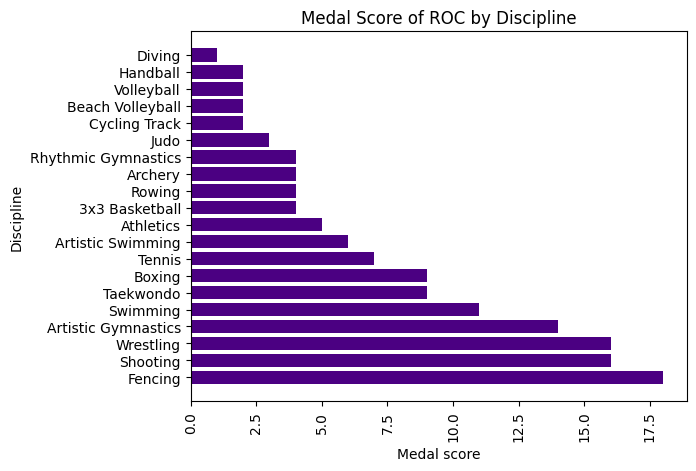
\includegraphics[width=0.75\linewidth]{assets/perf_ROC.png}
    \caption{Score de médailles de la Russie par discipline}
    \label{fig:enter-label}
\end{figure}

Nous appliquons ici un poids aux médailles, mais différent de celui utilisé dans les classements officiels. De plus, nous utilisons le fichier medals, où les médailles de chaque athlète sont renseignées : cela pose donc un problème pour les évènements collectifs, puisque un pays ayant une médaille dans un de ces évènements en aura en fait autant que d'athlètes dans l'équipe. Pour résoudre ce problème, il faut donc regrouper les médailles des évènements collectifs.
\\\indent Nous avons décidé d'étudier l'impact de la Russie dans les classements des 5 premières disciplines : escrime, tir, lutte, gymnastique artistique et natation.
\\\indent Tout d'abord, pour essayer d'évaluer cet impact, nous pouvons simplement étudier les classements dans ces 5 disciplines en 2020 et 2024. Cette fois, nous utiliserons la méthode de classement des JO, qui place en premier le pays ayant le plus de médailles d'or, puis de médailles d'argent si égalité, etc. Nous devons donc, à partir du fichier medals.csv, extraire un dataframe qui donne par pays et par discipline, le nombre de médailles d'or, d'argent, de bronze. Nous observons alors que les pays dans le top 5 pour chacune des 5 disciplines varient grandement. En effet, les équipes qualifiées changent chaque année, surtout pour les pays hôtes comme dit plus haut, donc les classements aussi. Nous aurions pu espérer voir un classement simplement décalé (le deuxième devient premier,...) que nous aurions alors pu facilement interpréter. Ici il est difficile de lier la non-participation de la Russie avec les variations observées. Nous voyons tout de même que le nombre de médailles gagnées par la Russie, même si elle n'est pas placée en tête de classement dans les 5 disciplines, reste notable. Elle pourrait donc influencer le classement si ses médailles revenaient à d'autres pays.
\\\indent Nous pouvons également essayer de mesurer cet impact grâce au modèle précédent. Au lieu d'exclure la Russie car elle ne participe pas aux JO 2024, nous gardons les données concernant ses athlètes, afin de prévoir un classement hypothétique si la Russie avait participé. Le rang de la Russie au sein de ce classement n'est pas ce qui nous intéresse. En effet, nous pourrions comparer les rangs des pays autres que la Russie avec leur classement réel lors des JO 2024. L'utilisation du modèle est la même, idem pour le pré-traitement des données, nous ne détaillerons donc pas. 
\\

\begin{figure}[H]
    \centering
    \begin{tabular}{|c|c|c|}
    \hline
        Rang & Prédit & Réel \\
        \hline
        1 & Afrique du Sud & Etats-Unis \\
        2 & Allemagne & Chine \\
        3 & Nigeria & Pays-Bas\\
        4 & Italy & France\\
        5 & Pays-Bas & Grande Bretagne\\
        6 & Brésil & Espagne\\
        7 & Bahamas &  Australie\\
        8 & Japon & Italie\\
        9 & Chine & Japon \\
        10 & Jamaïque & Nouvelle Zélande\\
    \hline
    \end{tabular}
    \caption{Comparaison classement prédit et classement réel Paris 2024}
    \label{tab:my_label}
\end{figure}

\subsection{Analyse des résultats}

Comme dit précédemment, bien que les résultats du modèle soient plutôt précis (~80\%), les classements globaux déduits de ces résultats ne le sont pas. Ici, nous obtenons un classement improbable, qui semble encore moins juste que lorsque nous excluions la Russie, nous ne pouvons donc pas interpréter ces résultats pour répondre à la question. 
\\\indent Tout ce que nous pouvons dire sur l'impact de la non-participation de la Russie est que le nombre de médailles par pays augmente globalement, comme dit plus haut. De plus, nous avons vu qu'il n'y avait pas de pays qui profitait particulièrement de l'absence de la Russie, nous pouvons donc supposer que les médailles remportées par les athlètes russes en 2020 ont été réparties entre beaucoup de pays, n'ayant pas un impact considérable sur le classement.

\section{Etude de la corrélation entre les variables socio-économiques et le succès aux JO 2024}

Enfin, nous allons nous intéresser à l'influence de certaines variables socio-économiques sur la réussite des pays aux Jeux Olympiques 2020 et 2024, qui sera ici quantifiée par le nombre total de médailles obtenues.

Pour ce faire, nous avons utilisé le dataset externe \href{https://www.kaggle.com/datasets/nelgiriyewithana/countries-of-the-world-2023}{Global Country Information Dataset 2023} qui regroupe des informations sur les pays telles que le PIB, la densité de population, le salaire minimum, etc.

\subsection{Pré-traîtement des données}

Nous devons tout d'abord relier nos données des JO (\verb|medals\_total.csv|) aux données du dataset utilisé. Comme certains noms de pays ne sont pas les mêmes dans les deux datasets (par exemple "ROC" pour "Russia"), nous commençons par mapper les noms des pays pour pouvoir ensuite merge les deux DataFrame. Nous observons que certains pays ne sont pas présents dans le dataset utilisé, comme Taipei ou le Kosovo, qui seront donc écartés de l'analyse. Nous écartons également les athlètes individuels neutres (AIN) et l'équipe olympique des réfugiés (EOR) qui ne représentent pas directement un pays.

Ensuite, les informations contenues dans le dataset utilisé ne sont pas bien formatées : il y a des symboles pourcent, dollar, et des virgules dans les nombres que nous aimerions utiliser. Nous reformatons alors les valeurs numériques et ne gardons que les colonnes numériques.

En ce qui concerne les données manquantes, nous utilisons une méthode d'imputation KNN qui va remplir les cases où nous n'avons pas de valeur en utilisant les valeurs des cinq plus proches voisins dans l'espace des données. Nous aurions pu utiliser d'autres techniques telles que la moyenne de la colonne, mais ça aurait pu amener à des valeurs absurdes si un tout petit pays se retrouvait avec par exemple un PIB de cent mille milliards de dollars (qui est la moyenne mondiale).
\\\\
\indent Nos données sont enfin prêtes à être utilisées dans un modèle prédictif qui mettra en évidence les relations entre le nombre total de médailles et les variables socio-économiques de chaque pays.

\subsection{Modèle}

Nous avons choisi d'utiliser un modèle d'arbre de régression qui, une fois entraîné sur l'ensemble des pays avec le nombre total de médailles comme cible, nous permettra d'examiner les différents splits choisis et de comprendre les corrélations entre les variables socio-économiques et la réussite de chaque pays aux JO 2020 et 2024.
\\

Le modèle d'arbre de régression est pratique car il ne suppose pas beaucoup de pré-conditions sur les données d'entrée et leur distribution. Ici nous avons décidé de limiter la profondeur maximale de l'arbre à 5 car l'idée était de voir les premiers splits sans trop rentrer dans les détails des splits finaux.
\\

Nous avons d'abord entraîné l'arbre sur les données de Tokyo, et nous avons obtenu un score R2 de plus de 97\% ainsi qu'une RMSE d'environ 3 médailles, ce qui est très correct et cela nous montre que l'arbre s'est bien adapté spécifiquement à notre jeu de données. L'idée n'était pas de faire un modèle généraliste qui pouvait prédire le nombre de médailles total pour un pays dans des JO différents (il serait en total overfit actuellement), mais bien de construire un modèle très spécifique qui met en évidence les corrélations pour nos données actuelles.
\\

Dans un deuxième temps, nous avons réentraîné l'arbre cette fois-ci sur les données des JO de Paris 2024, et avec un score R2 de plus de 98\% et une RMSE d'environ 2 médailles.
\\

Vous pouvez retrouver les version textuelles des deux arbres précédemment énoncés dans l'annexe \ref{annexe_arbres}.

\subsection{Résultats}

Nous observons tout d'abord que pour chacun des deux arbres obtenus, la première découpe se fait en fonction du PIB (GDP). En effet, pour Tokyo, les pays ayant un PIB inférieur à  2 771 milliards de dollars sont ceux dont le modèle prédit un petit nombre de médailles (moyenne estimée à 8 médailles totales), tandis que les pays ayant un PIB supérieur à cette somme sont estimés à un grand nombre de médailles (moyenne estimée à 72 médailles totales). Pour Paris, la division se fait à 2 663 milliards de dollars (moyenne de 7 médailles pour les pays inférieurs, et 70 médailles pour les pays supérieurs).
\\

Ensuite, pour les pays ayant un PIB inférieur à 2771 milliards de dollars aux JO de Tokyo, il y a un deuxième split sur le PIB situé à 1325 milliards de dollars (moyenne de 5 médailles pour les pays inférieurs, et 31 médailles pour les pays supérieurs). Dans la partie basse, c'est le salaire minimum qui fait la découpe, et dans la partie haute c'est l'indice des prix à la consommation (CPI). Pour les pays ayant un PIB supérieur à 2771 milliards de dollars, c'est le revenu des taxes qui sépare les deux groupes : nous observons une moyenne de 100 médailles pour les pays ayant un revenu des taxes inférieur à 10\% du PIB, et une moyenne de 53 médailles pour les pays ayant un revenu des taxes supérieur à 10\% du PIB.
\\

Aux JO de Paris, le salaire minimum fait la deuxième séparation parmi les pays ayant un PIB inférieur à 2663 milliards de dollars. Notre modèle prédit une moyenne de 5 médailles dans la partie basse, et une moyenne de 25 médailles dans la partie haute. Et pour les pays ayant un PIB supérieur à 2663 milliards de dollars, le groupe est séparé entre les pays dont le revenu des taxes est inférieur à 10\% du PIB (moyenne de 108 médailles prédite dans le groupe) et ceux dont le revenu des taxes est supérieur à 10\% du PIB (moyenne de 51 médailles prédite).

\subsection{Analyse des résultats}

Bien que nous n'ayons pas trouvé de dataset rassemblant des données sur les infrastructures sportives dans chaque pays (budget accordé, éducation sportive, etc.), ce sont des variables qui peuvent se déduire des facteurs vus précédemment.
\\

Nous pouvons tout d'abord remarquer que les pays ayant un PIB élevé réussissent généralement beaucoup mieux aux Jeux Olympiques que ce soit en 2020 ou 2024. Cela pourrait se comprendre de la manière suivante : les pays avec un fort PIB peuvent investir plus d'argent dans leur patrimoine culturel sportif et former plus de bons athlètes.
\\

Nous avons aussi vu que le salaire minimum, le revenu des taxes et l'indice des prix à la consommation sont de gros facteurs observés de réussite aux JO. En effet, nous pouvons ici faire l'hypothèse suivante : Les pays où les habitants ont un meilleur salaire, moins de taxes et un meilleur indice des prix à la consommation sont avantagés car les habitants ont plus de budget à consacrer à leur pratique sportive personnelle.
\\

Nous remarquerons en outre que les principaux critères de division entre les pays qui réussissent bien aux JO et ceux qui réussissent moins bien sont d'ordre économique. Si nous descendons plus profondément dans les arbres, nous trouverons également des splits sur le nombre de médecins par milliers d'habitants, ou encore le taux de natalité. Cependant, que ce soit à l'échelle du pays avec le PIB, ou à l'échelle des individus avec le salaire, il semble que ce soit toujours l'argent qui prime sur la réussite aux JO.

\section{Conclusion}
En conclusion, ce projet nous a permis de mettre en pratique nos compétences en traitement des données et intelligence artificielle sur un cas concret. Nous avons tout d’abord réalisé une analyse observatoire générale qui portait sur la répartition de certains critères chez les athlètes, puis par l'utilisation d'une méthode de clustering, nous avons identifié différents "types" de pays participants tels que les pays spécialisés ou encore les pays performants. \\

Ensuite, l'étude de l'évolution des classements entre 2020 et 2024 nous a poussé à créer un modèle nous permettant de prédire un classement grâce aux médailles prédites des athlètes participants. Ce modèle semble relativement performant lorsqu'il s'agit des résultats des athlètes, mais cela est dû au grand nombre d'athlètes ne remportant pas de médailles, le modèle ne prend donc pas de risque en prédisant un résultat de 0 médailles pour beaucoup d'athlètes. C'est pourquoi le classement prévu est assez différent du classement réel des JO Paris 2024. \\

En etudiant les variations dans le classement, nous pouvons nous intéresser particulièrement à la non-participation de la Russie et comment cela a impacté les résulats de Paris 2024. En utilisant des méthodes statistiques ainsi que le modèle précedent, il est difficile de mesurer cet impact, nous avons conclu qu'aucun pays particulier n'a profité de la non-participation de la Russie, mais plutôt l'ensemble des pays participants. \\

Enfin, nous nous sommes intéressés aux critères socio-économiques qui influencent la réussite aux JO. Les plus importants sont le PIB, le salaire minimum, le revenu des taxes et l'indice des prix à la consommation. En somme, les pays ayant le plus d'argent ou qui laissent le plus d'argent à leurs habitants réussissent mieux, ce qui semble logique. En effet, ces pays et leurs habitants ont plus d'argent à investir dans le sport.
\appendix

\clearpage
\section*{Annexes}
\addcontentsline{toc}{section}{Annexes}
\renewcommand{\thesubsection}{\Alph{subsection}}

\subsection{Pourcentage d’athlètes médaillés en fonction du nombre de disciplines médaillées en 2020 et 2024}
\label{annexe_athletes_disciplines}

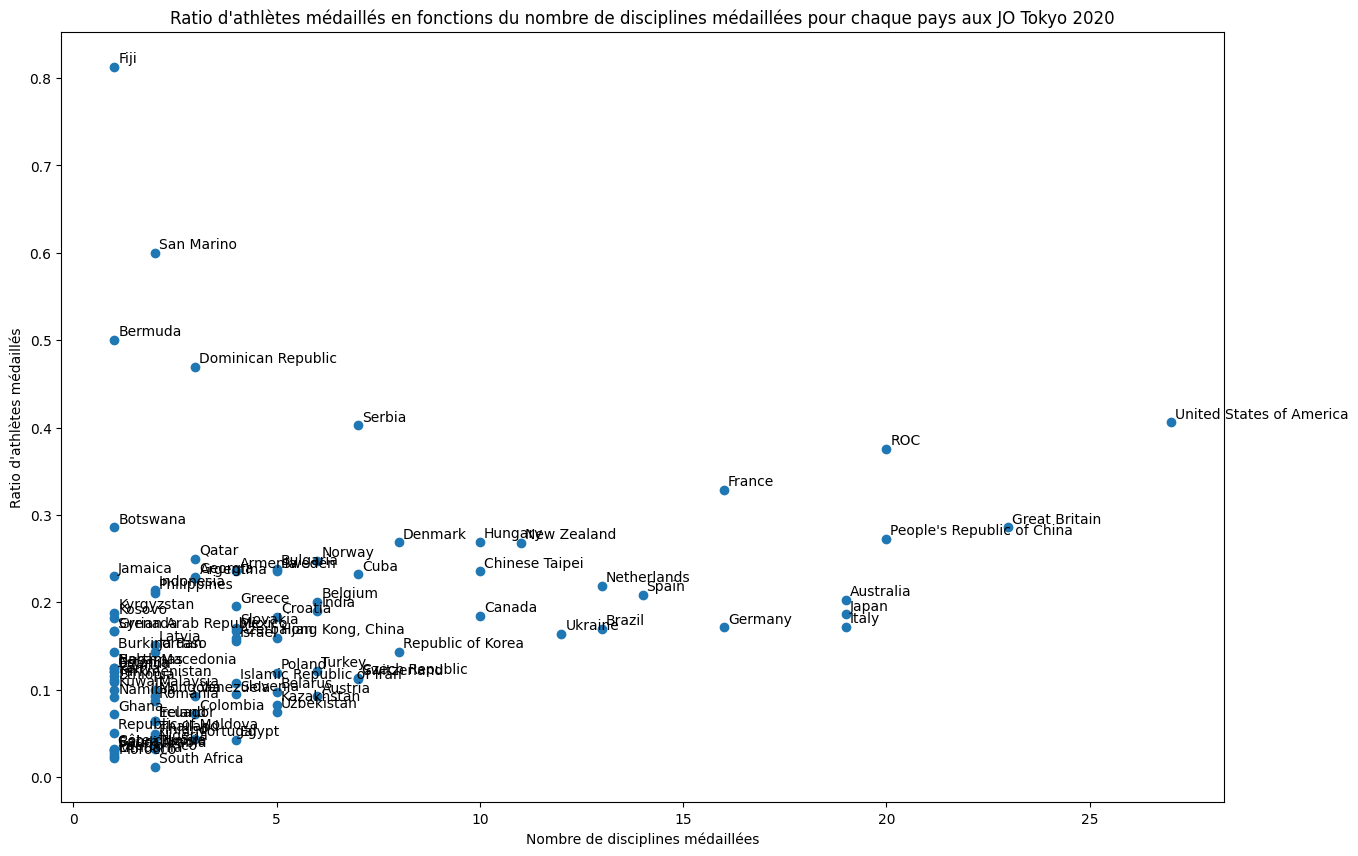
\includegraphics[width=\linewidth]{assets/athletes_disciplines_2020}

\hfill

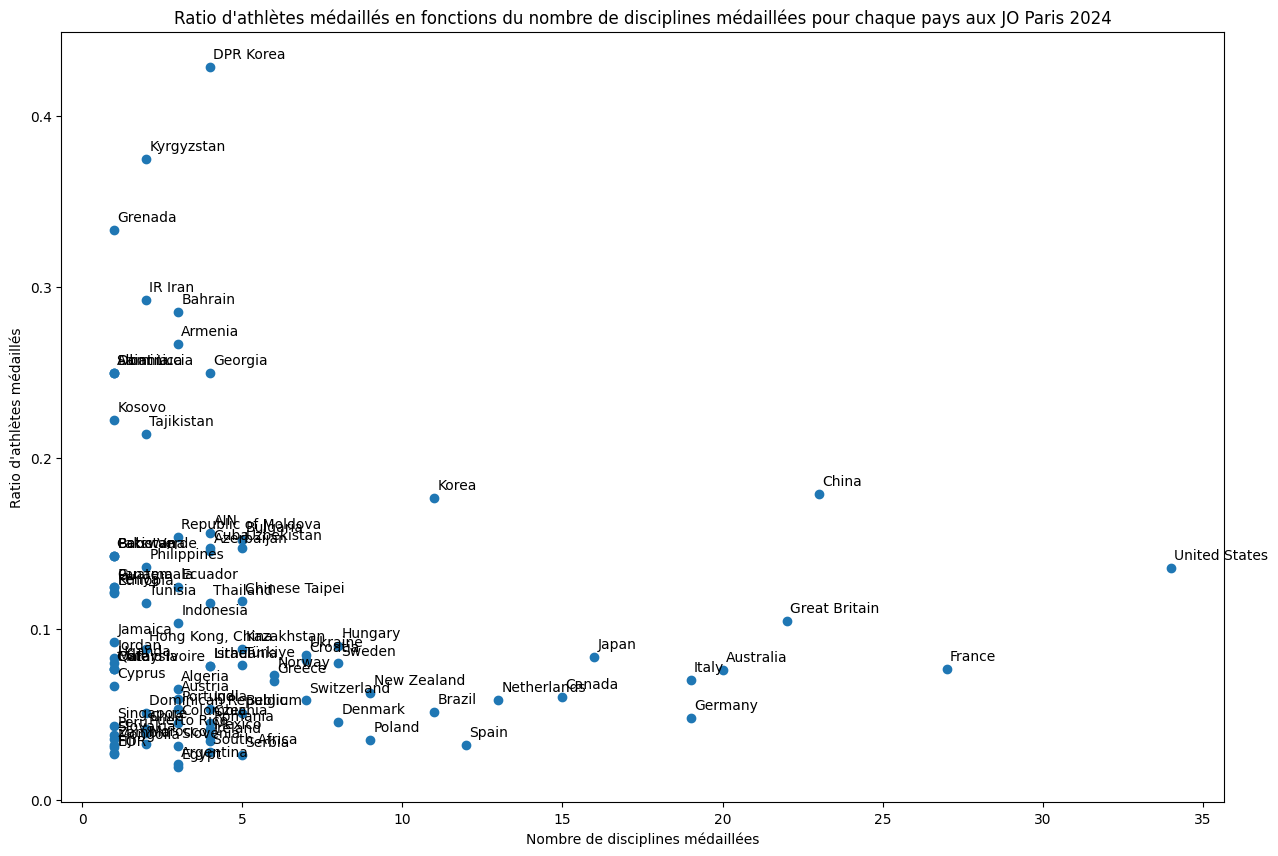
\includegraphics[width=\linewidth]{assets/athletes_disciplines_2024.png}

\clearpage
\subsection{Clusters identifiés par KMeans pour le pourcentage d'athlètes médaillés en fonction du nombre de disciplines médaillées en 2020 et 2024}
\label{annexe_athletes_disciplines_clusters}

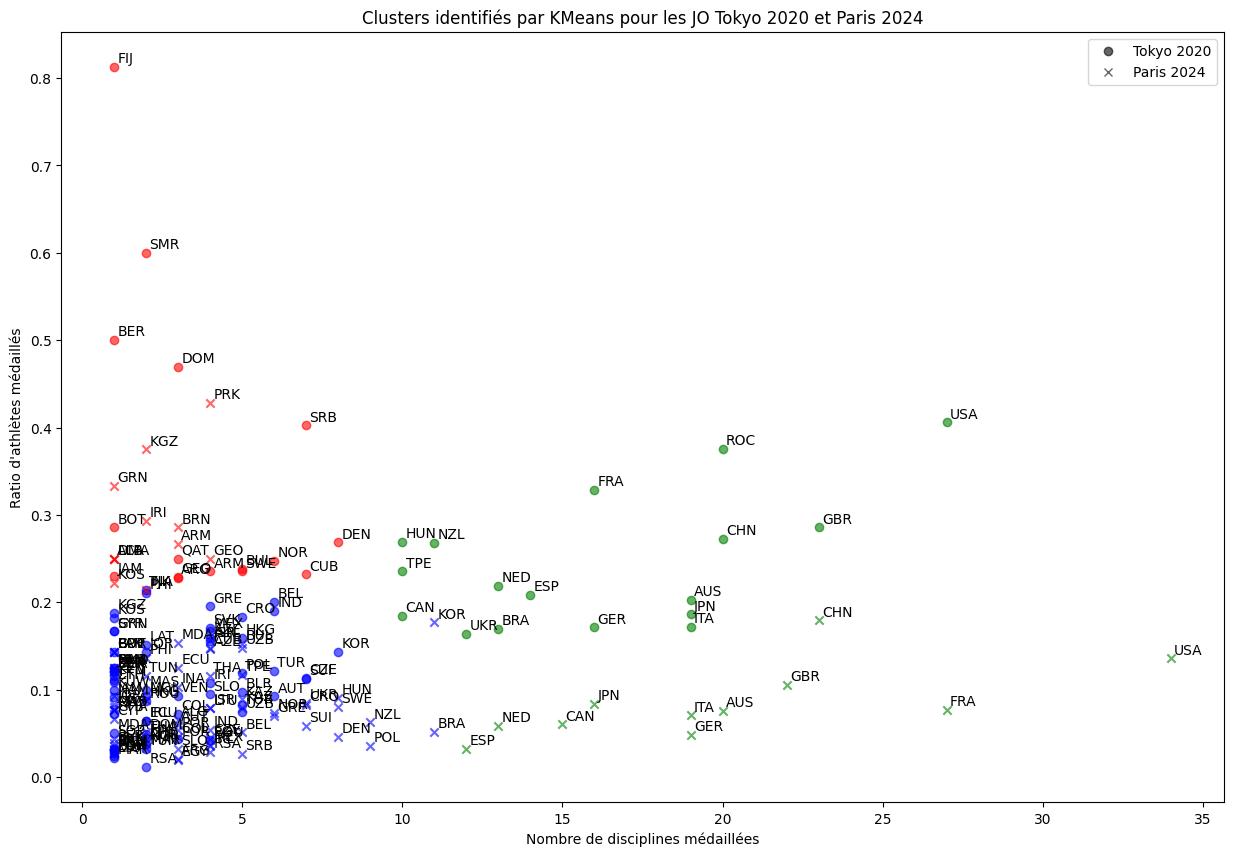
\includegraphics[width=\linewidth]{assets/athletes_disciplines_clusters.png}

\clearpage
\subsection{Comparaison \& différence du nombre total de médailles par pays (ordre croissant par rapport aux JO de Tokyo)}
\label{annexe_comp_nb_total_medailles_par_pays}

\begin{figure}[H]
    \center
    
    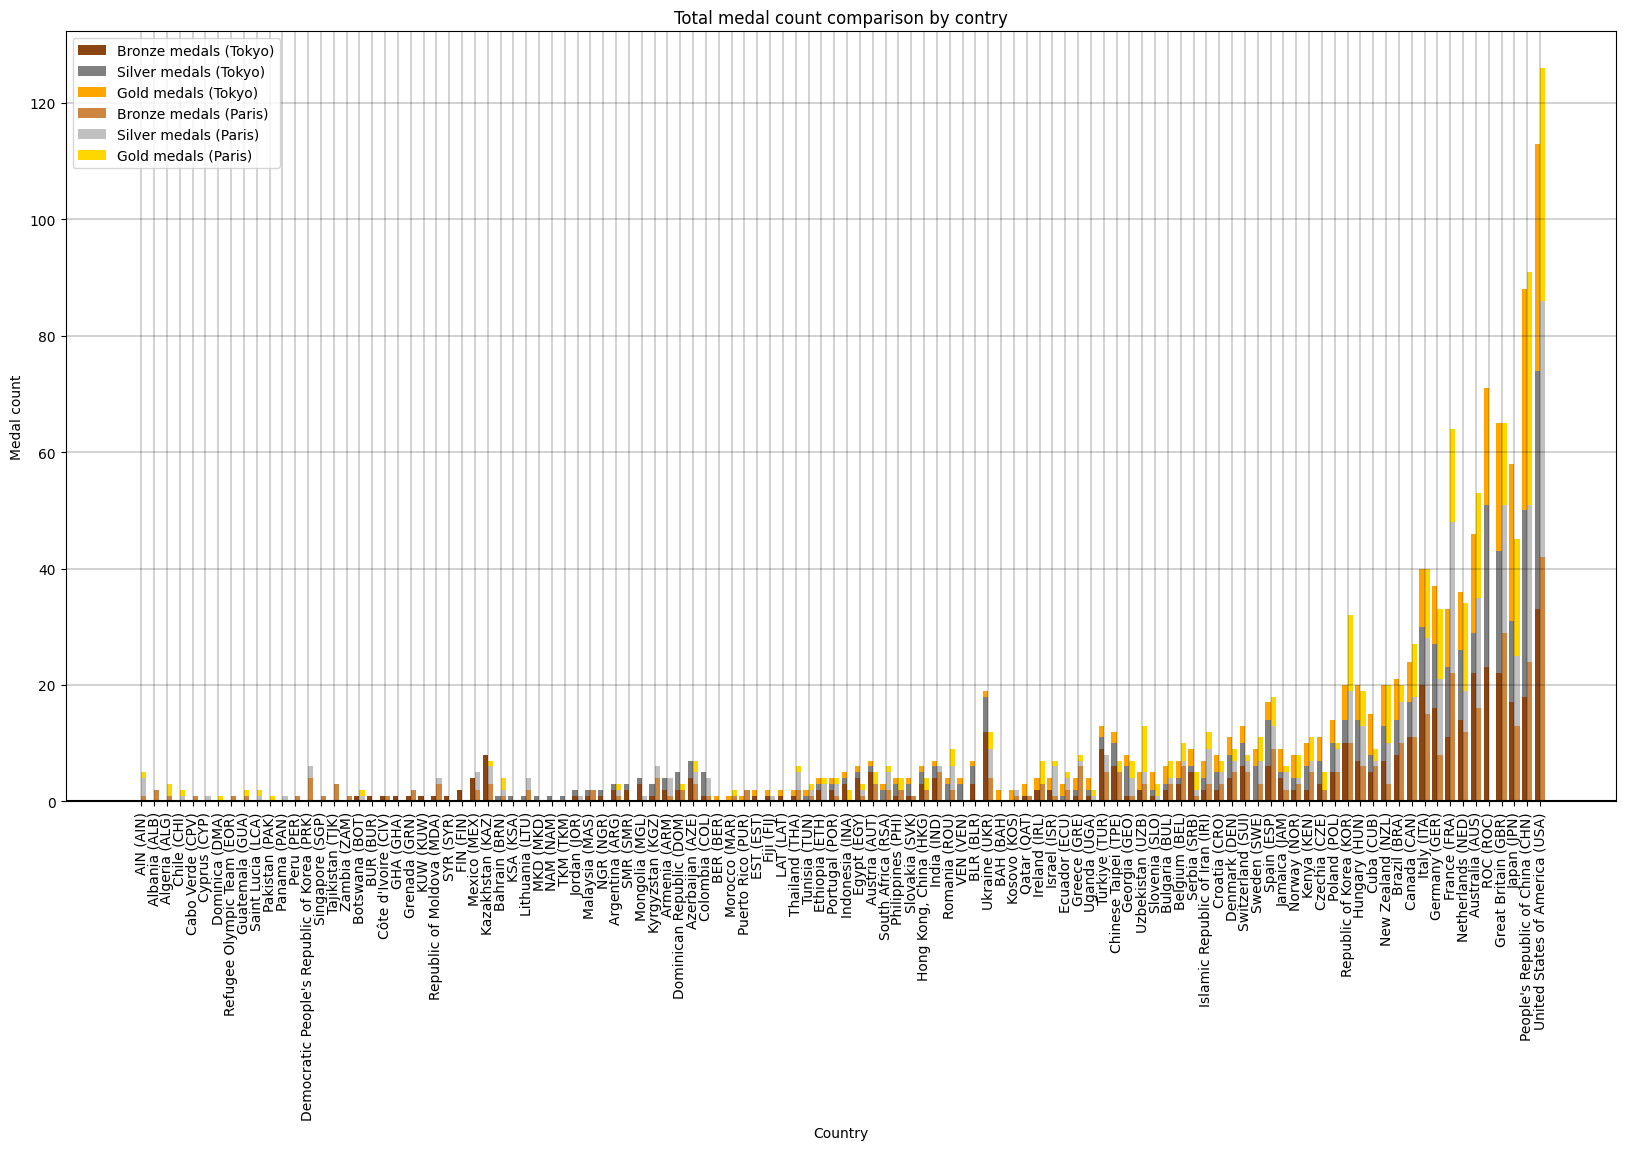
\includegraphics[width=1.0998\linewidth]{assets/comp_nb_total_medailles_par_pays.png}
\end{figure}

\begin{figure}[H]
    \center
    
    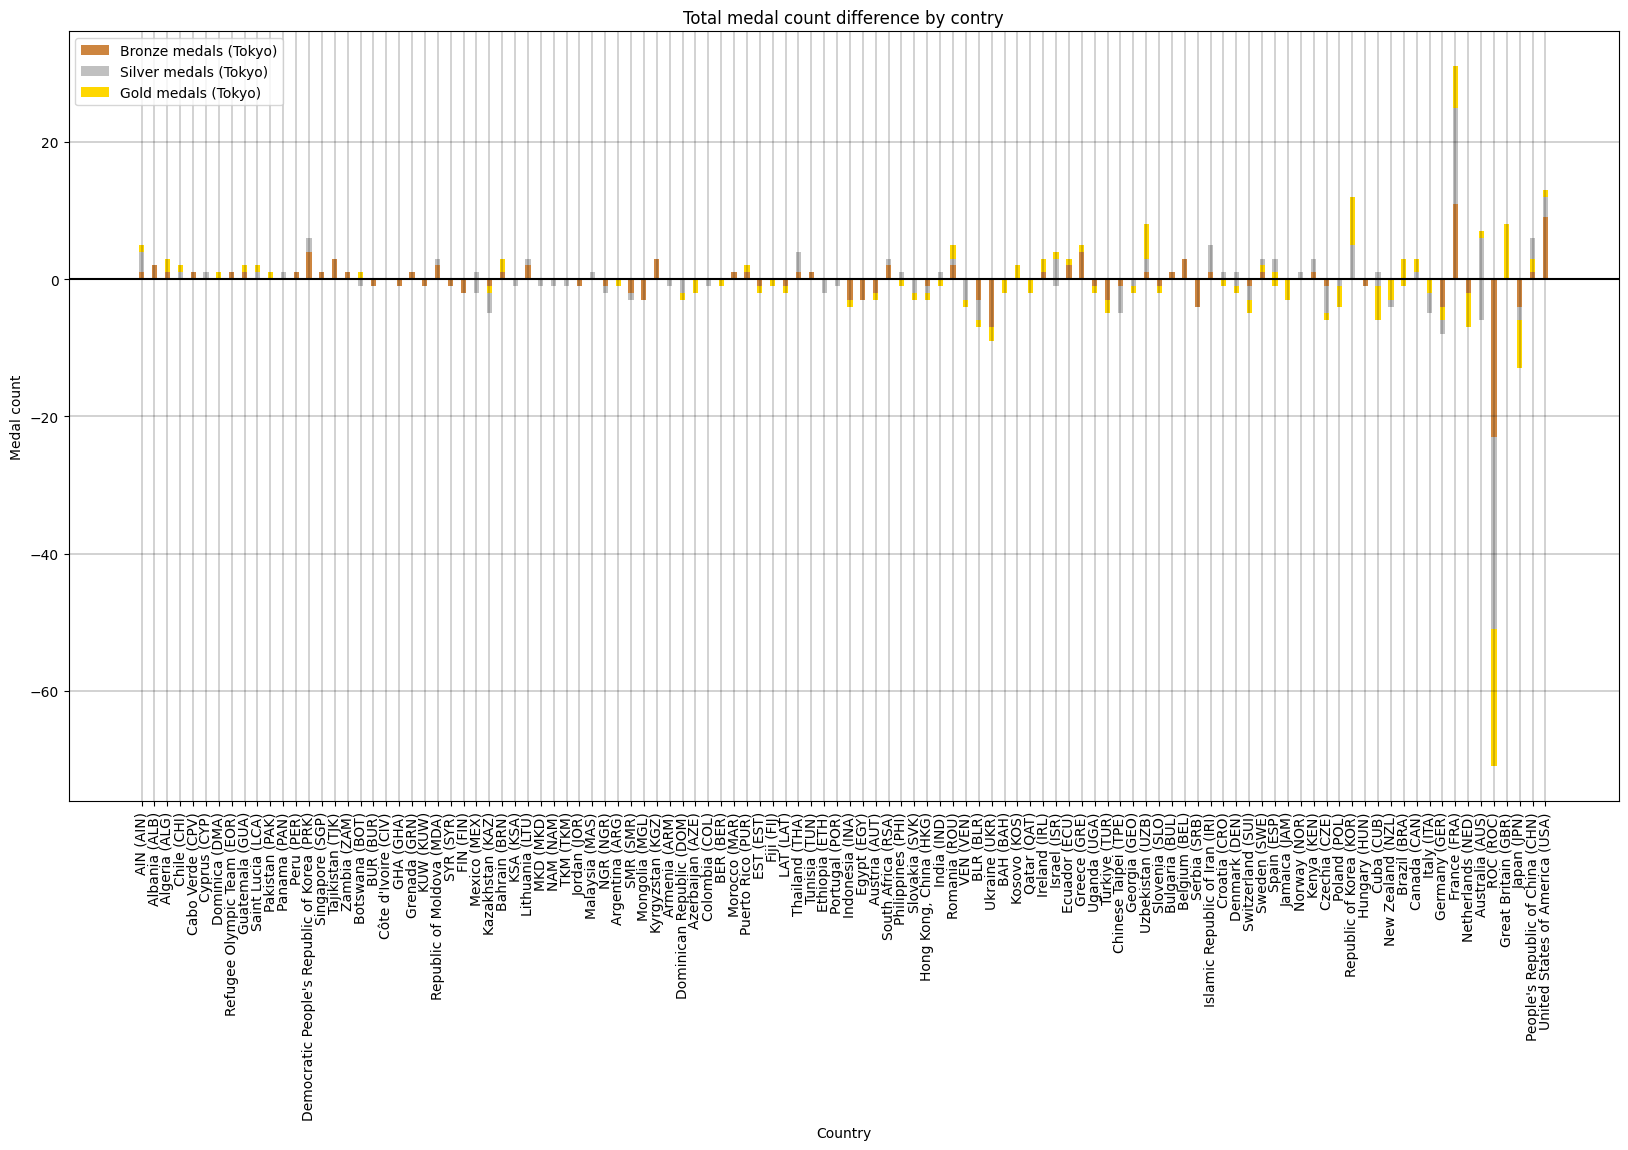
\includegraphics[width=1.0998\linewidth]{assets/diff_nb_total_medailles_par_pays.png}
\end{figure}

\clearpage
\subsection{Arbres de régression pour les critères socio-économiques}
\label{annexe_arbres}

\begin{lstlisting}[caption=Arbre sur les données de 2020]
|--- GDP <= 2771315720192.00
|   |--- GDP <= 1325483687936.00
|   |   |--- Minimum wage <= 8.93
|   |   |   |--- Birth Rate <= 16.28
|   |   |   |   |--- Population <= 5669433.50
|   |   |   |   |   |--- value: [3.76]
|   |   |   |   |--- Population >  5669433.50
|   |   |   |   |   |--- value: [9.47]
|   |   |   |--- Birth Rate >  16.28
|   |   |   |   |--- GDP <= 77962465280.00
|   |   |   |   |   |--- value: [1.94]
|   |   |   |   |--- GDP >  77962465280.00
|   |   |   |   |   |--- value: [4.22]
|   |   |--- Minimum wage >  8.93
|   |   |   |--- Out of pocket health expenditure <= 13.90
|   |   |   |   |--- Total tax rate <= 37.90
|   |   |   |   |   |--- value: [20.00]
|   |   |   |   |--- Total tax rate >  37.90
|   |   |   |   |   |--- value: [36.00]
|   |   |   |--- Out of pocket health expenditure >  13.90
|   |   |   |   |--- Forested Area (%) <= 16.80
|   |   |   |   |   |--- value: [4.00]
|   |   |   |   |--- Forested Area (%) >  16.80
|   |   |   |   |   |--- value: [7.00]
|   |--- GDP >  1325483687936.00
|   |   |--- CPI <= 180.60
|   |   |   |--- Tax revenue (%) <= 19.30
|   |   |   |   |--- Tax revenue (%) <= 12.00
|   |   |   |   |   |--- value: [7.00]
|   |   |   |   |--- Tax revenue (%) >  12.00
|   |   |   |   |   |--- value: [20.50]
|   |   |   |--- Tax revenue (%) >  19.30
|   |   |   |   |--- Fertility Rate <= 1.81
|   |   |   |   |   |--- value: [43.00]
|   |   |   |   |--- Fertility Rate >  1.81
|   |   |   |   |   |--- value: [33.00]
|   |   |--- CPI >  180.60
|   |   |   |--- value: [71.00]
|--- GDP >  2771315720192.00
|   |--- Tax revenue (%) <= 10.55
|   |   |--- Physicians per thousand <= 2.29
|   |   |   |--- value: [88.00]
|   |   |--- Physicians per thousand >  2.29
|   |   |   |--- value: [113.00]
|   |--- Tax revenue (%) >  10.55
|   |   |--- Population: Labor force participation (%) <= 61.25
|   |   |   |--- value: [37.00]
|   |   |--- Population: Labor force participation (%) >  61.25
|   |   |   |--- Maternal mortality ratio <= 6.00
|   |   |   |   |--- value: [58.00]
|   |   |   |--- Maternal mortality ratio >  6.00
|   |   |   |   |--- value: [65.00]

\end{lstlisting}

\clearpage
\begin{lstlisting}[caption=Arbre sur les données de 2024]
|--- GDP <= 2663259176960.00
|   |--- Minimum wage <= 6.05
|   |   |--- GDP <= 1326201503744.00
|   |   |   |--- Physicians per thousand <= 2.34
|   |   |   |   |--- Population <= 47304518.00
|   |   |   |   |   |--- value: [2.27]
|   |   |   |   |--- Population >  47304518.00
|   |   |   |   |   |--- value: [5.55]
|   |   |   |--- Physicians per thousand >  2.34
|   |   |   |   |--- Urban_population <= 4162730.50
|   |   |   |   |   |--- value: [3.70]
|   |   |   |   |--- Urban_population >  4162730.50
|   |   |   |   |   |--- value: [7.95]
|   |   |--- GDP >  1326201503744.00
|   |   |   |--- Agricultural Land( %) <= 56.50
|   |   |   |   |--- Total tax rate <= 56.05
|   |   |   |   |   |--- value: [18.00]
|   |   |   |   |--- Total tax rate >  56.05
|   |   |   |   |   |--- value: [20.00]
|   |   |   |--- Agricultural Land( %) >  56.50
|   |   |   |   |--- value: [6.00]
|   |--- Minimum wage >  6.05
|   |   |--- Co2-Emissions <= 133834.50
|   |   |   |--- Density
(P/Km2) <= 45.00
|   |   |   |   |--- value: [20.00]
|   |   |   |--- Density
(P/Km2) >  45.00
|   |   |   |   |--- Co2-Emissions <= 81027.50
|   |   |   |   |   |--- value: [7.00]
|   |   |   |   |--- Co2-Emissions >  81027.50
|   |   |   |   |   |--- value: [10.00]
|   |   |--- Co2-Emissions >  133834.50
|   |   |   |--- Minimum wage <= 11.94
|   |   |   |   |--- Physicians per thousand <= 3.79
|   |   |   |   |   |--- value: [31.00]
|   |   |   |   |--- Physicians per thousand >  3.79
|   |   |   |   |   |--- value: [40.00]
|   |   |   |--- Minimum wage >  11.94
|   |   |   |   |--- value: [53.00]
|--- GDP >  2663259176960.00
|   |--- Tax revenue (%) <= 10.55
|   |   |--- Tax revenue (%) <= 9.50
|   |   |   |--- value: [91.00]
|   |   |--- Tax revenue (%) >  9.50
|   |   |   |--- value: [126.00]
|   |--- Tax revenue (%) >  10.55
|   |   |--- Agricultural Land( %) <= 50.05
|   |   |   |--- GDP <= 4463699689472.00
|   |   |   |   |--- value: [33.00]
|   |   |   |--- GDP >  4463699689472.00
|   |   |   |   |--- value: [45.00]
|   |   |--- Agricultural Land( %) >  50.05
|   |   |   |--- GDP <= 2771315720192.00
|   |   |   |   |--- value: [64.00]
|   |   |   |--- GDP >  2771315720192.00
|   |   |   |   |--- value: [65.00]
\end{lstlisting}


\end{document}